\section{Background and Related Work}
\label{sec:related}
%\emph{\color{red}Related work including a short section of foundational work in the area of your thesis, a section on directly relevant work and how your proposed work either leverages that work (e.g., techniques you plan to adopt) or differs from it (e.g., novel contributions), and a description of how your proposed work is distinct from the work being done by your colleagues at UW.}
We begin by providing some background information on 802.11n Wi-Fi technology and the standard access point networks used in homes today. This background knowledge is useful to frame the discussion.

We next consider three classes of techniques to improve performance in Wi-Fi networks. There are mechanisms to optimize configuration of a single wireless link, mechanisms to optimize configuration for multiple links with concurrent workloads, and alternative network designs.

\subsection{Background}

\begin{table}
\centering
%\footnotesize
\begin{tabular}{ccc}
\toprule
Modulation & Coding Rate & Data Rate (Mbps) \\
\midrule
BPSK & 1/2 & 6.5 \\
QPSK & 1/2 & 13.0\\
QPSK & 3/4 & 19.5\\
QAM-16 & 1/2 & 26.0\\
QAM-16 & 3/4 & 39.0\\
QAM-64 & 2/3 & 52.0\\
QAM-64 & 3/4 & 58.5\\
QAM-64 & 5/6 & 65.0\\
\bottomrule
\end{tabular}
\caption{\label{tab:siso_mcs} 802.11n single-stream rates.}
%The single-stream 802.11n modulation and coding schemes. The first seven rates correspond to 802.11a/g rates (excluding 9\Mbps) with four added OFDM subcarriers; the highest data rate uses a new 5/6-rate code.}
\end{table}

\subsubsection{802.11n}
Our work applies to 802.11a/g/n radios that use coded Orthogonal Frequency Division Multiplexing (OFDM). 20 or 40\MHz channels are divided into 312.5\kHz bands called subcarriers, each of which sends independent data simultaneously. Convolutional coding is applied across the bits for error correction and bits are interleaved to spread them in frequency. 
Each subcarrier in a packet is modulated equally, using BPSK, QPSK, QAM-16, or QAM-64, with 1, 2, 4 or 6 bits per symbol, respectively. 
The data rates depend on the combination of modulation and coding. 

Our experimental platform uses 802.11n radios that operate on 20\MHz or 40\MHz channels.
The single-stream 802.11n rates are shown in \tabref{tab:siso_mcs}. 
The main innovation in 802.11n is the use of multiple antennas for  \emph{spatial multiplexing}. By using MIMO processing, multiple streams can be sent at the same time, each at the single-stream rate, for higher overall rates. Note that the details of single-stream 802.11n differ slightly from 802.11a/g (optimized coding rates and more data subcarriers), but in ways that are not material for our work so that we can treat 802.11n as a superset of 802.11a/g.

Choosing between the 8 different encodings in \tabref{tab:siso_mcs}, 2 channel widths, and up to 4 spatial streams implies at least 64 potential points in the operating space of a link, and this only represents the rate selection task. Thus, algorithms to configure 802.11n links have to make decisions from a much wider search space than the for 802.11a which only had 8 monotonically faster and harder to receive rates. 

Additionally, the capabilities of commercial 802.11n devices can vary wildly. The most powerful NICs commonly available have four or more antennas and support up to 600\Mbps rates. These devices have 540\MHz of spectrum available for connections: there are 3 orthogonal 20\MHz channels in the 2.4\GHz band, and 24 orthogonal channels in the 5\GHz band. Lower end devices work only on the three 2.4\GHz channels and can thus only use a total of 60\MHz of spectrum. These devices only use a single antenna, and support a maximum of 150\Mbps bitrates. Other devices can only transmit one spatial stream (150\Mbps in the best case) but can receive two streams and up to 300\Mbps. The wide variety in device capabilities means that links are truly asymmetric---one device may be significantly more powerful than the other, and link speeds may be fundamentally different depending on which node is transmitting.

This summarizes the basic properties of 802.11n that algorithms must be able to handle.

\subsubsection{Access point networks} The type of network most commonly used in the home is an \emph{access point network}~\cite{80211,nagus_homerf} (\figref{fig:ap_network}). The network is organized in a star topology, with the AP at the root and all clients operating on the same channel. The AP has a (typically wired) uplink connection to the Internet gateway, such as a DSL, FiOS, WiMAX, or cable modem. Topologically, the access point model provides a simple abstraction: it ignores the broadcast nature of wireless networks, and instead acts as an Ethernet switch (for the wireless LAN) and either an Ethernet bridge or IP router (for the uplink). The AP (or the network behind it) represents a central point for admission control, including IP configuration via DHCP, and DNS and NAT services. As if all the connections were wired, all transmissions from clients are sent to the AP, which routes these transmissions as appropriate, either back onto the wireless LAN for wireless clients, and otherwise out of the uplink connection. The primary constraint imposed by wireless is that, network wide, there can only be one ongoing transmission at a time. This is enforced by a simple CSMA/CA~\cite{karn_maca} mechanism and the optional use of RTS/CTS when there exist hidden terminals in the network.

\heading{Power save mode.}
In 802.11, access points also include specialized functionality that allows clients to conserve energy by putting their RF hardware to sleep. The AP buffers downlink packets for sleeping clients, which poll the AP for new traffic when they wake. When any client is asleep, the AP also buffers multicast and broadcast traffic, offloading these periodically every few beacons, typically with a period 200\ms--400\ms. However, the standard Wi-Fi contract mandates that the AP never sleeps---clients can contact the AP to send data or poll for traffic at any time.

\heading{Network extenders.}
Note that in large homes, the access point may have insufficient range. Thus the standard generalizes the star topology slightly to allow for wireless repeaters that act as Ethernet bridges to extend the AP network. These repeaters operate on the same channel as the AP and broadcast the same BSSID\@. They also offer the same contract as APs: they perform buffering for sleeping clients, and are not allowed to sleep themselves.

\heading{Wireless distribution system.}
\label{sec:wds}
In some networks there are be multiple access points that are connected via a wireless backbone. This is commonly the case in enterprise environments, in which APs are deployed as gateways for mobile to the larger wired LAN\@. In the home, some companies now offer ``dual band'' APs that include two NICs and act as two logical APs using the same SSID, one each on the 2.4\GHz and 5\GHz frequency bands. Dual band functionality maintains support for cheap devices that only operate on 2.4\GHz---which is often plagued by interference from microwaves, Bluetooth, and neighboring LANs---while allowing highly capable devices to use the 5\GHz frequency band which includes 24 non-interfering channels and provides better isolation from neighboring networks. In both these cases, the wireless access point networks operate as described above, independently and without cross-AP coordination, and only communicate via the wired backplane.

\heading{Network discovery.}
To join a wireless network, a client first conducts a scan by hopping through the available 802.11 channels and sending on each a link-layer broadcast packet called a Probe Request. Devices that offer network functionality, i.e.\ APs or extenders, respond to these probe requests with information about the network (SSID, AP MAC address, type of security, etc.) and a list of their capabilities (e.g., the bandwidth of the channel and the number of MIMO streams that the AP supports). A client selects between responding devices via local policy, but in practice clients simply select the AP with the strongest measured signal strength, or preferentially select the 5\GHz network when it meets a minimum signal strength threshold.

\heading{Summary.} Access point networks provide a simple wireless switch abstraction that works well, and this has driven the dramatic growth of Wi-Fi that continues today. However, as applications in the wireless home become more demanding, AP networks will be limited by their inability to support more efficient communication patterns when possible and their spectrally inefficient use of only one channel. We believe that a more flexible network is needed to enable these applications.

\begin{figure}[p]
      \centering
      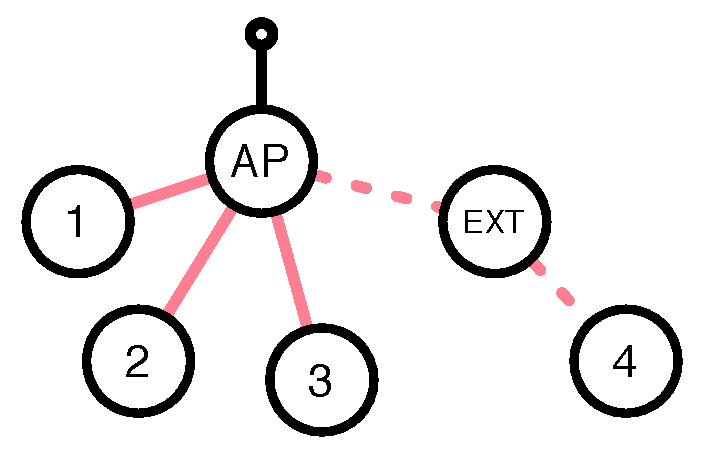
\includegraphics[width=0.8\columnwidth]{figures/omni/ap.pdf}
      \caption{\label{fig:ap_network} An access point network is structured as a star topology in which all nodes communicate on the same channel and talk directly to the access point. Optionally, wireless extenders can act as repeaters for distant clients (dashed lines) on the same channel.}
\end{figure}
\begin{figure}[p]
      \centering
      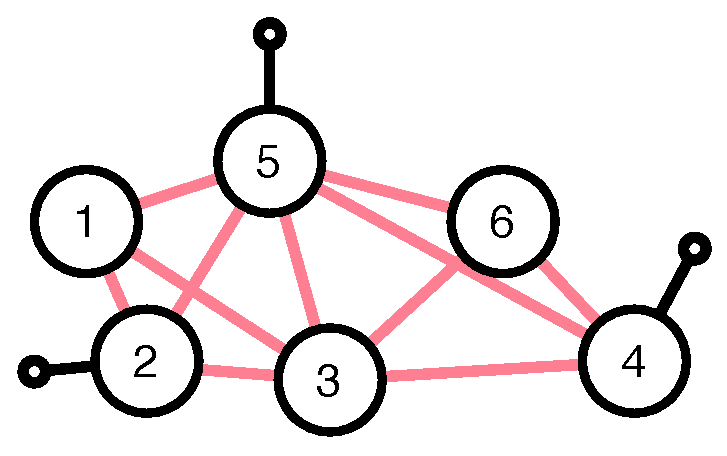
\includegraphics[width=0.8\columnwidth]{figures/omni/mesh.pdf}
      \caption{\label{fig:mesh} An mesh network is an unstructured topology in which any nodes on the same channel can communicate. There may be multiple egress points to external networks. In most work, the mesh uses a single channel, though in some cases (not pictured), nodes with two or more radios can use multiple channels.}
\end{figure}
\begin{figure}[p]
      \centering
      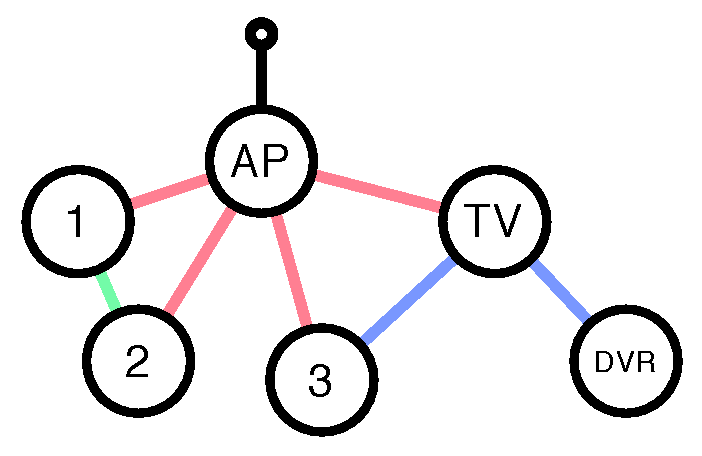
\includegraphics[width=0.8\columnwidth]{figures/omni/p2p.pdf}
      \caption{\label{fig:wifi_p2p} A Wi-Fi Direct ``peer-to-peer'' network enables devices to concurrently act as clients in one access point-like network while serving as members of another. Thus device-to-device communications, e.g., between nodes 1 and 2 or between the TV and DVR can happen directly and on different channels, hence different contention domains, than other ongoing communications.}
\end{figure}

\subsection{Configuring a Single Link}
An important first step towards operating a wireless network efficiently is operating an individual wireless link efficiently. The most basic challenge is rate adaptation, the task of selecting the best transmit modulation, coding rate, antennas, and number of spatial streams that fits the underlying RF channel. There are other important single link configuration problems---such as selecting the best frequency for the link, or trying to minimize the power consumption of one endpoint---but rate selection is the studied problem in this area since a good scheme has a large effect on throughput.

In theory, it is simple to select the physical layer configuration because this is directly determined by the specifics of the RF channel. The signal-to-noise ratio (SNR) is the gold standard for performance in narrowband channels. Textbook formulas relate the error rate of different modulations to the SNR~\cite{Tse}. The best rate, channel, or transmit power is then simple to compute.

In practice, 802.11 LANs have never used channel measurements as more than a coarse indicator of expected performance. There have simply been too many ways in which the observed measurements and actual performance fail to match the predictions of theory. For example, the most accessible channel measurement is received signal strength indication (RSSI), which serves as a proxy for the true SNR\@. RSSI measurements are samples that may vary over packet reception, be mis-calibrated, or be corrupted by interference, all of which are known to be issues in practice~\cite{camp_mobicom08, judd_rate_adapt, reis_sigcomm06}. Even if RSSI were perfect, it does not reflect the frequency-selective fading of 802.11 channels, which are not close to narrowband. Nor does it account for imperfect receivers that may greatly degrade performance~\cite{aguayo_roofnet,judd_rate_adapt}. Due to these factors, the minimum RSSI at which a rate starts to work varies by more than 10\dB for real links~\cite{reis_sigcomm06, snr_infocom08, zhao_sensys03}.

Instead, a form of guided search is widely used in practice to select operating points. Packet delivery is simply tested for a rate or transmit power to see how well it works. If the loss rate is too high, a lower rate is used, otherwise a higher rate is tested. Lucent's ARF algorithm~\cite{lucent_arf}, OAR~\cite{sadeghi_oar}, and SampleRate~\cite{Bicket_SampleRate} were early rate adaptation algorithms of this type. The state of the art today is the Linux kernel's Minstrel~\cite{minstrel}, a version of SampleRate adapted for modern Wi-Fi hardware that can use lower rates for packet retransmissions. Minstrel has also been adapted for 802.11n, performing parallel searches between the multiple MIMO modes with different numbers of spatial streams and channel bandwidths. The guided search approach is very effective for slowly varying channels and simple configurations (e.g., a few rates with fixed transmit power and channel) since the best setting will soon be found.

For rapidly varying channels, these algorithms become less effective. Camp, et al.~\cite{camp_mobicom08} demonstrated the importance of varying the time constants used to generate summary statistics for Minstrel-like algorithms. Recently, RapidSample~\cite{ravindranath_sensorhints} used hints from smartphone sensors to detect mobility and switch to a simplified SampleRate-like algorithm that walks up and down the rates in an agile manner. This provides better performance when devices are moving, but it is not obvious how to extend RapidSample's logic to 802.11n where there is not a single linear set of rates.

%However, search becomes less effective as channels change more quickly and the configuration space becomes more complex. Both of these factors are trends: 802.11 clients are increasingly used when they are truly mobile, both walking and in vehicles; and NICs that are now being deployed with 802.11n depend on multiple antennas, which adds another dimension to and increases the size of the search space. Also, tuning combinations such as rate and power is much more complex. 

Recent work has returned to the theoretical approach and made headway by measuring symbol-level details of packet reception. In particular, SoftRate uses the output of soft-Viterbi decoding for each symbol to estimate the bit error rate (BER)~\cite{Vutukuru_SoftRate}. This allows it to predict the effects on packet delivery of changing the rate. AccuRate uses symbol error vectors for the same purpose~\cite{accurate_nsdi10}.  However, these methods are not defined for selecting other useful parameters, such as transmit power, and they do not extend from 802.11a/g to 802.11n, e.g., when selecting antennas or numbers of spatial streams.

\heading{Summary.}
%In theory, RF channel measurements should enable the endpoints of a link to determine useful parameters such as rate, MIMO mode, antennas, operating channel, and transmit power levels. However, the RF measurements available from commodity Wi-Fi cards are inadequate for good performance in practice. Instead, Wi-Fi uses guided search algorithms in practice, but these can complex and inefficient in rapidly varying channels. Recent work at the physical layer has moved back towards theoretical algorithms, but these are not available in hardware today and may not extend to 802.11n.
In a wireless home with competing workloads and fluctuating topology, the configuration of a single link is a small sub-problem, yet important to solve accurately and rapidly to ease the burden of higher-layer decisions. Today's algorithms are effective for static links, but likely insufficient when devices are mobile or for tasks such as selecting the best intermediary or best operating channel. As part of our thesis, we provide a better solution that works on commodity 802.11n NICs available today (\secref{sec:preliminary}).

\subsection{Managing Multiple Links}
There are many ways to manage multiple competing workloads in the literature. In the 802.11 access point model, all workloads use the same channel and take turns sending. Here we discuss some problems with this approach, and three different types of solutions.

\subsubsection{Reducing Single-Channel Anomalies}
One notable problem with the standard 802.11 MAC protocol is termed the \emph{rate anomaly problem}~\cite{heusse_anomaly} in which a slow link usurps an unfair proportion of the airtime and degrades performance for the rest of the network. This is a well-studied problem that results from the MAC's allocation of access to the medium on a per-packet basis, rather than a per-time basis. One practical approach to alleviating rate anomaly is to use a repeater~\cite{bahl_repeater}. The intuition behind this approach is that a well placed relay can more than double the speed of a really slow link, and thus reduce the amount of airtime consumed by that sender even if the relayed packet must be sent twice in order to reach its destination. This concept of relaying has other benefits, including reduced power consumption the distant device spends less time sending~\cite{bahl_multiradio}. It also extends to pipelines in multihop networks~\cite{rodrig_thesis}. These pipelines can be further improved if nodes use multiple radios and hence can make use of multiple channels~\cite{bahl_multiradio}.

There is another tactic for alleviating the rate anomaly problem, and that is to have nodes compete for the medium on a per-time basis. This has been implemented in Wi-Fi in the form of 802.11e~\cite{80211} block transmissions, and this mechanism was subsequently improved in 802.11n~\cite{80211n}. Still, the other benefits of repeaters in Wi-Fi networks remain applicable to our home networks.

Katti, et al.~\cite{katti_xors} applied network coding to wireless network to improve the performance of the MAC when multiple wireless flows cross through the same node, e.g., the access point in a home network. Network coding provides a gain of around 1.5 in the common case, but unbounded in some corner cases due to MAC issues. However, the same 802.11e/n mechanisms that alleviate rate anomaly reduce the network coding gain back down to around 1.5 to 2. Also, the extant system designs cover only networks that use a single rate, whereas 802.11n has many rates and antenna configurations to choose form, and fundamentally different, heterogeneous links. This work might be applicable to home wireless networks with bidirectional workloads, but the machinery is fairly complicated and probably of little gain in practice.

\subsubsection{Spatial Reuse: Concurrent Links on a Single Channel}
There is a wide body of work that aims to achieve spatial reuse, that is the ability of devices in the network to concurrently transmit on the same channel, but controlled in such a way as to allow receivers to successfully receive their intended packets. CMAP~\cite{vutukuru_cmap} measures a conflict map between links that enables each sender to decide whether it can interfere with an ongoing transmission without hurting other receivers. Successive interference cancellation~\cite{halperin_sic} leverages capture---the reception of a strong transmission over a weaker one---in a receiver with the ability to subtract out the captured interference signal to recover the weaker transmission to improve performance for ZigBee networks. Other work modifies CSMA/CA by tuning transmit power levels, carrier sense thresholds, and selecting rates carefully~\cite{kim_tuning}. A third class of work uses directionality to improve capacity, either by using physically directional beams to reduce the spread of a transmission~\cite{liu_dirc} or careful beamforming to diagonalize a channel, in the case of Multiuser MIMO~\cite{heath_mumimo,spencer_mumimo}.

These works all fundamentally change the access primitive in the wireless network away from simple CSMA/CA. Though some of these techniques, such as tuning all the parameters to match a cellular network, or successive interference cancellation, and multiuser MIMO are capacity-achieving in theory, all these techniques result in a gain of at most 2$\times$ in theory, and this may be overstated in practice~\cite{brodsky_csma}. In our opinion, even the best case improvement still represents a fairly small gain over much simpler mechanisms that can work in the hardware we have today. 

\subsubsection{Leveraging multiple channels}
Finally, there is work that leverages multiple channels to improve network performance. The 1980's Ethernet M-LANs~\cite{marsan_multichan}, the late 1990's work on Multichannel CSMA~\cite{nasipuri_multichan}, and more recent work on Wi-Fi with variable channel width~\cite{chandra_chanwidth} showed that by splitting the available spectrum into subchannels, MAC level efficiency can be dramatically improved because it separates concurrent transmissions into isolated contention domains. More recently, FICA~\cite{tan_fica} showed that a similar subchannel approach can be used to improve MAC efficiency by reducing collisions when many nodes want to send on the same channel.

For fast networks such as 802.11n, MAC overheads can grow large and isolating nodes into different contention domains can offer a big improvement. Interestingly, the M-LANs and Multichannel CSMA work assumed that all available spectrum was utilized, and split among multiple channels; however the more recent Wi-Fi work taking the same approach has instead subdivided a single Wi-Fi channel into subchannels. This improved performance for contention in the single channel, but recall that in 802.11n there are 27 orthogonal channels, of which an AP network can only use a single one. We believe it likely that the performance improvements will be much more dramatic by taking advantage of a larger slice of the available spectrum, a decision that was taken for granted in the original work and since forgotten.

Recent implementation efforts have made progress towards enabling multichannel operation for a single network. In particular,  MultiNet~\cite{chandra_multinet} and FatVAP~\cite{kandula_fatvap} are two projects that enabled a client to associate to multiple simultaneous networks for a variety of purposes. 

\heading{Summary:} Of many mechanisms for managing contention among multiple workloads in a network, we find the most practical mechanisms for home networks to be those that maintain the basic contracts of the network, including CSMA/CA as MAC and the assumption of only one transmission in the network on any given frequency. With the improved efficiency hinted at by work using multiple channels instead to isolate competing workloads while at the same time reducing overhead, and the huge number of available channels, we believe that using multiple channels offers the most practical opportunity for improvement. The use of multiple channels complements nicely the practical repeater mechanism of Bahl, et al.\ discussed above. We conclude that these two methods are the most important first methods to examine when trying to improve home networks. Next, we consider alternate network architectures for Wi-Fi networks to see how they match up with our vision of the future wireless home.

\subsection{Alternate Network Architectures}
Finally, we consider the three main alternative designs for wireless networks that differ from the Wi-Fi access point model.

\subsubsection{Mesh networks}
The second type of wireless network is a mesh network (\figref{fig:mesh}). In a mesh, the nodes are spread over a much larger area and offer Internet service to clients that are typically separated from gateways by several hops~\cite{whitehead_mesh}. Two instance of this include Rice University's TFA project~\cite{camp_tfa,rice_tfa}, which provides Internet connectivity to low income urban neighborhoods in Houston, and Meraki~\cite{meraki}, which provides wireless coverage for hotels. There are also research mesh networks, such as Roofnet~\cite{bicket_roofnet}, which study the generalized problem of routing traffic in many directions across a mesh without a specific application.

The main problems in mesh networks are caused by their large spread and resulting many-hop paths. For instance, much of the research on mesh networks focuses on maintaining a distributed routing infrastructure~(e.g., \cite{draves_ett,rozner_soar}), pipelining transfers along long mesh paths~\cite{li_blockswitched,li_mesh,rodrig_thesis}, using network coding to improve performance of crossing flows~\cite{katti_xors,katti_anc}, or propagating data more effectively across the network by making use of many unreliable links~\cite{biswas_exor}. As a result of the complex nature of these solutions, work on mesh networks tends to simplify other aspects of network design, for instance by using homogenous single-antenna nodes, or fixing the entire network to a single bitrate.

\heading{Summary.} In our view, mesh networks are poorly matched to the home. The hard problems in mesh revolve around the sparsity of nodes, low quality of links, and long paths. In contrast, the constrained spacing and dense deployment of devices will make paths in the home likely to be short---at most a few hops---and of high bandwidth, which should be manageable by simpler mechanisms. Instead, the problems that mesh work ignores, such as heterogeneous devices and rate adaptation, are likely to be the hard problems in the home.
 
\subsubsection{Wi-Fi Direct: peer-to-peer networks}
The third type of wireless network is a Wi-Fi Direct ``peer-to-peer'' network~\cite{wifi_direct} (\figref{fig:wifi_p2p}), which represents a middle ground between the logically centralized access point networks and the logically distributed mesh networks. The groundwork for these networks was laid by Chandra, et al.\ in MultiNet~\cite{chandra_multinet}, which enabled a client to connect to multiple APs concurrently. MultiNet virtualizes a single wireless device across multiple access points, keeping one virtual client active at a time. Inactive virtual clients in MultiNet enable power save to force APs to buffer their traffic, and in this manner, all virtual clients can maintain associativity to their respective APs. When the hardware permits fast frequency switching, MultiNet clients can even associate to APs on different channels. In the original implementation of MultiNet, only one virtual client could be active at a time, even when two operated on the same channel, because the hardware could only be programmed to associate to a single AP at a time.

In essence, Wi-Fi Direct offers a standardized, updated MultiNet interface with better device support. In particular, some NICs can be programmed with multiple BSSIDs in order to operate virtual devices on the same channel concurrently. Second, hardware manufacturers have made fast channel switching a priority, with some NICs able to switch between channels on different bands within 2\ms~\cite{atheros_ar9390}. Finally, Wi-Fi Direct better handles the case where one NIC acts as a virtual client in one network and the access point for another. If these operate on different channels, the virtual access point will have to sleep while the virtual client is active, thereby violating the standard Wi-Fi contract that access points are always available. Thus Wi-Fi Direct adds mechanisms for a virtual AP to notify clients of its absence.

\heading{Summary.} We believe that Wi-Fi Direct supports many of the protocol mechanisms we would need to build a flexible home network. For instance, it should be possible to use multiple virtual devices to build a single logically-connected network that looks like an extended access point network, but makes uses of multiple channels to separate independent device-to-device workloads. We also believe it is possible to extend these mechanisms to support short-circuited paths in the network. However, as with rate selection in 802.11n, \emph{Wi-Fi Direct provides no instruction as to how to make decisions} about when to initiate the use of multiple channels; what devices, which links, and what operating channels to choose; or how to manage the network in a distributed manner. These are among the challenges we propose to tackle in this work.

\subsubsection{Cellular networks}
Finally, cellular data networks, in particular 4G networks based on WiMAX~\cite{wimax} or LTE/LTE-Advanced~\cite{lte}, offer wireless data service over a wide (metropolitan scale) area. These networks are highly centralized, and include scheduling mechanisms to tightly control and optimize the timing, frequency use, and rate of all transmissions in the network. The purpose of a WiMAX network is not for device-to-device communication, but rather device-to-Internet. In general, the cellular data networks do not provide a suitable model to replicate in the home.